%
% Module 3 Chapter 6 Homework
% CSC160-C00: Computer Science I (C++)
% Author: Ashton Hellwig
%


\documentclass[a4paper, 10pt]{article}


  % Packages
  \usepackage[utf8]{inputenc}       % Encoding
  \usepackage[english]{babel}       % Internationalization
  \usepackage{soul}                 % Highlighting
  \usepackage{hyperref}             % Links (internal and external)
  \usepackage{fancyhdr}             % Headers and footers
  \usepackage[dvipsnames]{xcolor}   % Text Colors
  \usepackage{listings}             % Code Snippets
  \usepackage{algorithm}            % For TOC support
  \usepackage{algorithmicx}         % Algorithmic notation support
  \usepackage{algpseudocode}        % Algorithmic notation environments
  \usepackage{enumitem}             % Ordered lists
  \usepackage{geometry}             % Page layout
  \usepackage{graphicx}             % Image support
  \usepackage[toc, page]{appendix}  % Appendix
  \usepackage{bookmark}
  \usepackage{adjustbox}
  \usepackage{csquotes}
  \usepackage{amsthm}
  \usepackage{array}
  \usepackage{makecell}
  \usepackage{amsmath}
  \usepackage{amssymb}
  \usepackage{relsize}
  \usepackage{multicol}
  \usepackage{etoolbox,refcount}
  \usepackage{parcolumns}

  \UseRawInputEncoding

  % Tables
  \renewcommand\theadalign{bc}
  \renewcommand\theadfont{\bfseries}
  \renewcommand\theadgape{\Gape[4pt]}
  \renewcommand\cellgape{\Gape[4pt]}

  % Lists
  \newcounter{countitems}
  \newcounter{nextitemizecount}
  \newcommand{\setupcountitems}{%
    \stepcounter{nextitemizecount}%
    \setcounter{countitems}{0}%
    \preto\item{\stepcounter{countitems}}%
  }
  \makeatletter
  \newcommand{\computecountitems}{%
    \edef\@currentlabel{\number\c@countitems}%
    \label{countitems@\number\numexpr\value{nextitemizecount}-1\relax}%
  }
  \newcommand{\nextitemizecount}{%
    \getrefnumber{countitems@\number\c@nextitemizecount}%
  }
  \newcommand{\previtemizecount}{%
    \getrefnumber{countitems@\number\numexpr\value{nextitemizecount}-1\relax}%
  }
  \makeatother    
  \newenvironment{AutoMultiColItemize}{%
  \ifnumcomp{\nextitemizecount}{>}{3}{\begin{multicols}{2}}{}%
  \setupcountitems\begin{itemize}}%
  {\end{itemize}%
  \unskip\computecountitems\ifnumcomp{\previtemizecount}{>}{3}{\end{multicols}}{}}



  % Colors
  \newcommand{\commentstylecolor}{\color{Gray}}
  \newcommand{\keywordstylecolor}{\color{MidnightBlue}}
  \newcommand{\stringstylecolor}{\color{ForestGreen}}
  \newcommand{\questioninput}{\color{Red}}
  \newcommand{\answertcolor}{\color{Green}}
  \newcommand{\myanswer}{\answertcolor{\hl}}

  % Symbols
  \newcommand{\answerflow}{\rotatebox[origin=c]{180}{$\Lsh$}}
  \newcommand{\toanswer}{\mathlarger{\mathlarger{\answerflow}}\quad}

  % Math
  \newcommand{\highlight}[1]{%
    \colorbox{green!50}{$\displaystyle#1$}}

  % Image Directory
  \graphicspath{ {screenshots/} }


  % Hyperlink Setup
  \hypersetup{
    colorlinks = true,
    urlcolor = blue,
    linkcolor = blue
  }


  % Syntax-Highlighting for Code Snippets
  \lstset{
    backgroundcolor=\color{white},
    breaklines=true,%
    captionpos=b,%
    frame=tb,%
    tabsize=4,%
    % numbers=left,%
    showstringspaces=false,%
    commentstyle=\commentstylecolor,%
    keywordstyle=\keywordstylecolor,%
    stringstyle=\stringstylecolor%
  }
  \lstset{literate=
  {á}{{\'a}}1 {é}{{\'e}}1 {í}{{\'i}}1 {ó}{{\'o}}1 {ú}{{\'u}}1
  {Á}{{\'A}}1 {É}{{\'E}}1 {Í}{{\'I}}1 {Ó}{{\'O}}1 {Ú}{{\'U}}1
  {à}{{\`a}}1 {è}{{\`e}}1 {ì}{{\`i}}1 {ò}{{\`o}}1 {ù}{{\`u}}1
  {À}{{\`A}}1 {È}{{\'E}}1 {Ì}{{\`I}}1 {Ò}{{\`O}}1 {Ù}{{\`U}}1
  {ä}{{\"a}}1 {ë}{{\"e}}1 {ï}{{\"i}}1 {ö}{{\"o}}1 {ü}{{\"u}}1
  {Ä}{{\"A}}1 {Ë}{{\"E}}1 {Ï}{{\"I}}1 {Ö}{{\"O}}1 {Ü}{{\"U}}1
  {â}{{\^a}}1 {ê}{{\^e}}1 {î}{{\^i}}1 {ô}{{\^o}}1 {û}{{\^u}}1
  {Â}{{\^A}}1 {Ê}{{\^E}}1 {Î}{{\^I}}1 {Ô}{{\^O}}1 {Û}{{\^U}}1
  {œ}{{\oe}}1 {Œ}{{\OE}}1 {æ}{{\ae}}1 {Æ}{{\AE}}1 {ß}{{\ss}}1
  {ű}{{\H{u}}}1 {Ű}{{\H{U}}}1 {ő}{{\H{o}}}1 {Ő}{{\H{O}}}1
  {ç}{{\c c}}1 {Ç}{{\c C}}1 {ø}{{\o}}1 {å}{{\r a}}1 {Å}{{\r A}}1
  {€}{{\euro}}1 {£}{{\pounds}}1 {«}{{\guillemotleft}}1
  {»}{{\guillemotright}}1 {ñ}{{\~n}}1 {Ñ}{{\~N}}1 {¿}{{?`}}1
}
  \newenvironment{alltt}{\ttfamily}{\par}


  % Page Configuration
  %% Style
  \pagestyle{fancy}

  %% Layout
  \geometry{%
  a4paper,%
  top=2.5cm,%
  bottom=2.5cm,%
  left=2.5cm,%
  right=2.5cm%
  }
  \setlength{\headheight}{12pt}
  \setlength{\floatsep}{12pt}

  %% Title page
  \title{Module 3 Chapter 6 Homework}
  \author{Ashton Hellwig}
  \date\today
  \setcounter{tocdepth}{3}

  %% Subsequent pages
  \lhead{CSC160}
  \rhead{Computer Science I (C++)}
  \lfoot{M3C6HW}
  \rfoot{A. Hellwig}

 
  % Document Content
\begin{document}
  \maketitle
  \tableofcontents
  \lstlistoflistings
  \newpage

  % Question 1
  \section{Question 1}
    Determine the value of each of the following expressions:
      \begin{enumerate}[label=\Alph*.]
        \item \lstinline[columns=fixed, language=c++]%
          {static_cast<char>(toupper('7'))}
        \item \lstinline[columns=fixed, language=c++]%
          {static_cast<char>(toupper('@'))}
        \item \lstinline[columns=fixed, language=c++]%
          {static_cast<char>(toupper('s'))}
        \item \lstinline[columns=fixed, language=c++]%
          {static_cast<char>(toupper('J'))}
        \item \lstinline[columns=fixed, language=c++]%
          {static_cast<char>(tolower('*'))}
        \item \lstinline[columns=fixed, language=c++]%
          {static_cast<char>(tolower(';'))}
        \item \lstinline[columns=fixed, language=c++]%
          {static_cast<char>(tolower('w'))}
        \item \lstinline[columns=fixed, language=c++]%
          {static_cast<char>(tolower('('))}
      \end{enumerate}
    % Question 1 Solution
    \subsection{Solution}
      \begin{enumerate}[label=\Alph*.]
        \item \lstinline[columns=fixed, language=c++]%
          {static_cast<char>(toupper('7'))} = \hl{7}
        \item \lstinline[columns=fixed, language=c++]%
          {static_cast<char>(toupper('@'))} = \hl{@}
        \item \lstinline[columns=fixed, language=c++]%
          {static_cast<char>(toupper('s'))} = \hl{S}
        \item \lstinline[columns=fixed, language=c++]%
          {static_cast<char>(toupper('J'))} = \hl{J}
        \item \lstinline[columns=fixed, language=c++]%
          {static_cast<char>(tolower('*'))} = \hl{*}
        \item \lstinline[columns=fixed, language=c++]%
          {static_cast<char>(tolower(';'))} = \hl{;}
        \item \lstinline[columns=fixed, language=c++]%
          {static_cast<char>(tolower('w'))} = \hl{w}
        \item \lstinline[columns=fixed, language=c++]%
          {static_cast<char>(tolower('('))} = \hl{(}
      \end{enumerate}

  % Question 2
  \section{Question 2}
    Consider the following function:

    \begin{lstlisting}[language=c++]
int mystery(int x, double y, char ch) {
  if (x == 0 && ch > 'A') 
    return(static_cast<int>(pow(y, 2)) + static_cast<int> (ch)); 
  else if (x > 0)
    return(x + static_cast<int>(sqrt(y)) - static_cast<int> (ch)); 
  else
    return(2 * x + static_cast<int>(y) - static_cast<int> (ch));
}
    \end{lstlisting}

    What is the output of the following C++ statements?
      \begin{enumerate}[label=\Alph*.]
        \item \lstinline[columns=fixed,language=c++]%
          {cout << mystery(0, 6.5, 'K') << endl;}
        \item \lstinline[columns=fixed,language=c++]%
          {cout << mystery(4, 16.0, '#') << endl;}
        \item \lstinline[columns=fixed,language=c++]%
          {cout << 2 * mystery(-11, 13.8, '8') << endl;}
      \end{enumerate}
    % Question 2 Solution
    \subsection{Solution}
      \begin{enumerate}[label=\alph*.]
        \item \lstinline[columns=fixed,language=c++]%
          {cout << mystery(0, 6.5, 'K') << endl;} = \hl{117}
        \item \lstinline[columns=fixed,language=c++]%
          {cout << mystery(4, 16.0, '#') << endl;} = \hl{-27}
        \item \lstinline[columns=fixed,language=c++]%
          {cout << 2 * mystery(-11, 13.8, '8') << endl;} = \hl{-130}
      \end{enumerate}

  % Question 3
  \section{Question 3}
    Consider the following program:

    \begin{lstlisting}[language=c++,numbers=left]
#include <iostream>
using namespace std; 

void func1(); 
void func2(); 

int main() { 
  int num;

  cout << "Enter 1 or 2: "; 
  cin >> num; 
  cout << endl;

  cout << "Take ";

  if (num == 1) 
    func1(); 
  else if (num == 2) 
    func2(); 
  else 
    cout << "Invalid input. You must enter a 1 or 2" << endl; 

  return 0; 
}

void func1() { 
  cout << "Programming I." <<endl;
}

void func2() { 
  cout << "Programming II." <<endl;
}
    \end{lstlisting}

    \begin{enumerate}[label=\Alph*.]
      \item What is the output if the input is 1?
      \item What is the output if the input is 2?
      \item What is the output if the input is 3?
      \item What is the output if the input is -1?
    \end{enumerate}
    % Question 3 Solution
    \subsection{Solution}
      \begin{table}[H]
        \resizebox{\textwidth}{!}{
        \begin{tabular}{||c|c||}
          \hline
          \textbf{Input} & \textbf{Output} \\ [0.5ex]
          \hline\hline
          1 & \hl{Take Programming I.} \\
          \hline
          2 & \hl{Take Programming II.} \\
          \hline
          3 & \hl{Take Invalid input. You must enter a 1 or 2} \\
          \hline
          -1 & \hl{Take Invalid input. You must enter a 1 or 2} \\
          \hline
        \end{tabular}}
      \end{table}


  \newpage
  % Question 4
  \section{Question 4}
    Consider the following program:

    \begin{lstlisting}[language=c++,numbers=left]
#include <cmath>
#include <iomanip>
#include <iostream>

using namespace std;

void traceMe(double x, double y);

int main() {
  double one, two;

  cout << "Enter two numbers: ";
  cin >> one >> two;
  cout << endl;

  traceMe(one, two);
  traceMe(two, one);
  return 0;
}

void traceMe(double x, double y) {
  double z;
  if (x != 0)
    z = sqrt(y) / x;
  else {
    cout << "Enter a nonzero number: ";
    cin >> x;
    cout << endl;
    z = floor(pow(y, x));
  }
  cout << fixed << showpoint << setprecision(2);
  cout << x << ", " << y << ", " << z << endl;
}
    \end{lstlisting}

    \begin{enumerate}[label=\Alph*.]
      \item What is the output if the input is 3 625?
      \item What is the output if the input is 24 1024?
      \item What is the output if the input is 0 196?
    \end{enumerate}
    % Question 3 Solution
    \subsection{Solution}
      \begin{table}[H]
        \resizebox{0.5\textwidth}{!}{
        \begin{tabular}{||l|l||}
          \hline
          \textbf{Input} & \textbf{Output} \\ [0.5ex]
          \hline\hline
          3 625 & \makecell{\hl{3.00, 6.25, 8.33} \\ \hl{625.00, 3.00, 0.00}} \\
          \hline
          24 1024 & \makecell{\hl{24.00, 1024.00, 1.33} \\%
            \hl{1024.00, 24.00, 0.00}} \\
          \hline
          0 196 & \makecell{\hl{Enter a nonzero number: 0 196} \\
            \hl{0.00, 196.00, 1.00} \\%
            \hl{196.00, 0.00, 0.00}} \\
          \hline
        \end{tabular}}
      \end{table}


  \newpage
  % Question 5
  \section{Question 5}
    Consider the following function definition:

    \begin{lstlisting}[language=c++]
void defaultParam(int num1, int num2 = 7, double z = 2.5) {
  int num3;
  num1 = num1 + static_cast<int>(z);
  z = num2 + num1 * z;
  num3 = num2 - num1;
  cout << "num3 = " << num3 << endl;
}
    \end{lstlisting}

    What is the output of the following function calls?
      \begin{enumerate}[label=\Alph*.]
        \item \lstinline[language=c++,columns=fixed]
          {defaultParam(7);}
        \item \lstinline[language=c++,columns=fixed]
          {defaultParam(8, 2);}
        \item \lstinline[language=c++,columns=fixed]
          {defaultParam(0, 1, 7.5);}
        \item \lstinline[language=c++,columns=fixed]
          {defaultParam(1, 2, 3.0);}
      \end{enumerate}
  % Question 5 Solution
    \subsection{Solution}
      \begin{enumerate}[label=\alph*.]
        \item \lstinline[language=c++,columns=fixed]
          {defaultParam(7);}

          \begin{lstlisting}[language=bash,caption=5a Solution]
num3 = -2
          \end{lstlisting}
        \item \lstinline[language=c++,columns=fixed]
          {defaultParam(8, 2);}

          \begin{lstlisting}[language=bash,caption=5b Solution]
num3 = -8
          \end{lstlisting}
        \item \lstinline[language=c++,columns=fixed]
          {defaultParam(0, 1, 7.5);}

          \begin{lstlisting}[language=bash,caption=5c Solution]
num3 = 6
          \end{lstlisting}
        \item \lstinline[language=c++,columns=fixed]
          {defaultParam(1, 2, 3.0);}

          \begin{lstlisting}[language=bash,caption=5d Solution]
num3 = -2
          \end{lstlisting}
      \end{enumerate}


  \newpage
  \appendix
  \section{Question 1}
    \begin{lstlisting}[language=c++,label={q1:listing},caption={Question 1 Implementation}]
#include <iostream>

using namespace std;

int main() {
  char a = static_cast<char>(toupper('7'));
  char b = static_cast<char>(toupper('@'));
  char c = static_cast<char>(toupper('s'));
  char d = static_cast<char>(toupper('J'));
  char e = static_cast<char>(tolower('*'));
  char f = static_cast<char>(tolower(';'));
  char g = static_cast<char>(tolower('w'));
  char h = static_cast<char>(tolower('('));

  cout << "a = " << a << '\n';
  cout << "b = " << b << '\n';
  cout << "c = " << c << '\n';
  cout << "d = " << d << '\n';
  cout << "e = " << e << '\n';
  cout << "f = " << f << '\n';
  cout << "g = " << g << '\n';
  cout << "h = " << h << endl;

  return 0;
}
    \end{lstlisting}
    \begin{figure}[H]
      \centering
      \caption{Listing \ref{q1:listing} Output}
      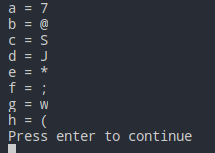
\includegraphics{q1output.png}
      \label{q1:output}
    \end{figure}
\end{document}